\documentclass[english,twoside, openright]{report}
\usepackage[utf8]{inputenc}
\usepackage{babel}
\usepackage{physics}
\usepackage{xcolor}
\usepackage{amsmath}
\usepackage{amsfonts}
\usepackage{lineno,hyperref}
\usepackage{hyperref}

\usepackage{tikz}
\usetikzlibrary{arrows, decorations.markings}

\tikzstyle{vecArrow} = [thick, decoration={markings,mark=at position
   1 with {\arrow[semithick]{open triangle 60}}},
   double distance=1.4pt, shorten >= 5.5pt,
   preaction = {decorate},
   postaction = {draw,line width=1.4pt, white,shorten >= 4.5pt}]
\tikzstyle{innerWhite} = [semithick, white,line width=1.4pt, shorten >= 4.5pt]

\newcommand{\cas}[2]{
  \mathcal{C}_{#1}\left[#2\right]
}
\newcommand{\Abs}[1]{
  \left|#1\right|
}

\newcommand{\wigsixj}[6]{
  \left\{
    \begin{matrix}
      #1 & #2 & #3 \\
      #4 & #5 & #6
    \end{matrix}
  \right\}
}
  

\author{Jamil KR}
\title{$U_p(4)\; \times\; U_q(4)$}
\begin{document}
\maketitle

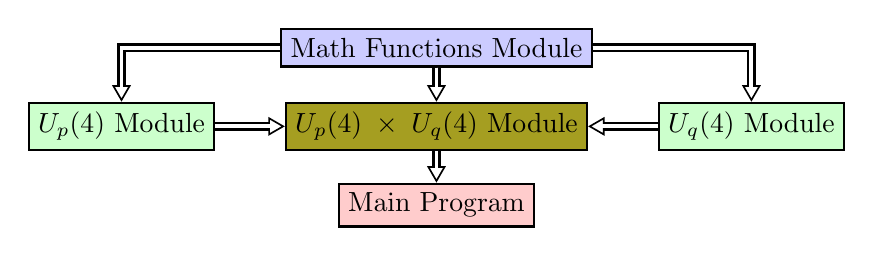
\begin{tikzpicture}[thick]
  \node[draw,rectangle,fill=green!20] at (-3,0)(a){$U_p(4)$ Module};
  \node[draw,rectangle,fill=olive!80,right of=a] at (0,0)(c){$U_p(4)\;\times\;U_q(4)$ Module};
  \node[draw,rectangle,fill=green!20,right of=c]at(4,0)(b){$U_q(4)$ Module};
  \node[draw,rectangle,fill=blue!20,above of=c](d){Math Functions Module};
  \node[draw,rectangle,fill=red!20,below of=c](e){Main Program};
  
  \draw[vecArrow] (a) to (c);
  \draw[vecArrow] (b) to (c);
  \draw[vecArrow] (d) to (c);
  \draw[vecArrow] (c) to (e);
  \draw[vecArrow] (d) -| (a);
  \draw[vecArrow] (d) -| (b);

  \draw[innerWhite] (a) to (c);
  \draw[innerWhite] (b) to (c);
  \draw[innerWhite] (d) to (c);
  \draw[innerWhite] (c) to (e);
  \draw[innerWhite] (d) -| (a);
  \draw[innerWhite] (d) -| (b);
\end{tikzpicture}

\section{Math Functions Module $\rightarrow$ \texttt{MOD\_matfun.f90}}

\begin{itemize}
\item Functions:
  \begin{itemize}
  \item \texttt{p\_symbol}(a,b) $=\; (a)_s\;=\;a(a+1)...(a+s-1)$
  \item \texttt{factorial}(n) $=\;n!$
  \item \texttt{delta\_function}(a,b,c) $=\;\Delta(\text{abc})$
  \item
    \texttt{wigner\_6j}$(j_1,j_2,j_3,l_1,l_2,l_3)\;=\;\wigsixj{j_1}{j_2}{j_3}{l_1}{l_2}{l_3}$
    \footnote{Definition of the book \textit{Nuclear Shell Theory} of
      Amos de-Shalit and Igal Talmi}
  \end{itemize}
\end{itemize}

\section{$U_p(4)$ Module $\rightarrow$ \texttt{MOD\_Up4.f90}}
Hamiltonian:

\begin{equation}
  \hat{H}_{U_p(4)} = \beta \; \cas{2}{so_p(4)} + \gamma \; \cas{2}{so_p(3)} + \gamma_2 \; \left[\cas{2}{so_p(3)}\right]^2 + \kappa \; \cas{2}{so_p(4)}\cas{2}{so_p(3)}
\end{equation}

\begin{itemize}
\item Global definitions:
  \begin{itemize}
  \item Npval: $U(4)$ Totally symmetric representation.
  \end{itemize}
\item Functions:
  \begin{itemize}
  \item Function: \texttt{RME\_Casimir\_SOp4}
  \item Function: \texttt{RME\_Casimir\_SOp3}
  \item Function: \texttt{RME\_Qp2}
  \end{itemize}
\end{itemize}

\section{$U_q(4)$ Module $\rightarrow$ \texttt{MOD\_Uq4.f90}}

Hamiltonian:

\begin{equation}
  \hat{H}_{U_q(4)} = a \; \cas{1}{u_q(3)} + b \; \cas{2}{u_q(3)} + c \; \cas{2}{so_q(3)} + d \; \cas{2}{so_q(4)}
\end{equation}

\begin{itemize}
\item Global definitions:
  \begin{itemize}
  \item Nqval: $U(4)$ Totally symmetric representation.
  \end{itemize}
\item Functions:
  \begin{itemize}
  \item Function: \texttt{RME\_Casimir\_Uq3}
  \item Function: \texttt{RME\_Casimir\_SOq3}
  \item Function: \texttt{RME\_Casimir\_SOq4}
  \item Function: \texttt{RME\_Qq2}
  \end{itemize}
\end{itemize}

\section{$U_p(4)\;\times\;U_q(4)$ Module $\rightarrow$ \texttt{MOD\_Up\_x\_Uq.f90}}

\begin{itemize}
\item Global definitions:
  \begin{itemize}
    \item
  \end{itemize}
\item Functions:
  \begin{itemize}
  \item Subroutine: \texttt{dimension\_po}
  \item Subroutine: \texttt{build\_basis\_po}
  \item Subroutine: \texttt{initialize\_position\_index}
  \item Function: \texttt{RME\_Qp\_x\_Qq\_0}
  \item Function: \texttt{RME\_Ip\_x\_SOq4}
  \item Subroutine: \texttt{build\_Up\_x\_Uq\_matrix}
  \item Function; \texttt{pretty\_braket}
  \end{itemize}
\end{itemize}

\subsection{Building the basis}

We have a block-diagonalizable system dividing the problem in para
($\text{mod}(J,2)=0$) and ortho ($\text{mod}(J,2)=1$) cases, and
separating by different $\Lambda$. The states will be stored in the
same array sorted by $\Lambda$. The dimension of each block will be
saved in \texttt{dim\_[SYM]}($\Lambda=0$), ... ,
\texttt{dim\_[SYM]}($\Lambda=\Lambda_{\text{max}}$).

\begin{align}
  \left.\left[
  \begin{array}{c}
    \ket{\psi_{1}^{\Lambda=0} }\\
    \vdots \\
    \ket{\psi_{\text{\texttt{dim\_[SYM]}}(\Lambda=0)}^{\Lambda=0}}
  \end{array}
  \right]\right\}& \rightarrow \text{1:\texttt{dim\_[SYM]}}(\Lambda=0)
  \nonumber\\
  \vdots  \qquad \qquad \qquad &
  \\
  \left.\left[
  \begin{array}{c}
    \ket{\psi_{1}^{\Lambda=\Lambda_{\text{max}}} }\\
    \vdots \\
    \ket{\psi_{\text{\texttt{dim\_[SYM]}}(\Lambda=\Lambda_{\text{max}})}^{\Lambda=\Lambda_{\text{max}}}}
  \end{array}
  \right]\right\}& \rightarrow \text{1:\texttt{dim\_[SYM]}}(\Lambda=\Lambda_{\text{max}}) \nonumber
\end{align}

Therefore, the basis array is as follow:

\begin{equation}
  \text{\texttt{basis\_[SYM]}}=\left[\ket{\psi_{1}^{\Lambda=0}},...,\psi_{\text{\texttt{dim\_[SYM]}}(\Lambda=0)}^{\Lambda=0},...,\ket{\psi_{1}^{\Lambda=\Lambda_{\text{max}}}},...,\psi_{\text{\texttt{dim\_[SYM]}}(\Lambda=\Lambda_{\text{max}})}^{\Lambda=\Lambda_{\text{max}}}\right]
\end{equation}

Each element of the the basis must cotain information about quantum numbers:

\begin{align}
  \ket{\psi_i^{\Lambda}}=\left(w\;J;\;n\;L;\;\Lambda\in\left[\Abs{J-L},J+L\right]\right)
\end{align}

\subsubsection{Dimension: \texttt{dimension\_po}}

Fortran90 subroutine.

\vbox{
Inputs:
\begin{itemize}
\item Npval. Integer
\item Nqval. Integer
\item $\Lambda_{\text{max}}$. Integer
\end{itemize}
}

\vbox{
Outputs:
\begin{itemize}
\item dim\_para. Integer, dimension(0:$\Lambda_{\text{max}}$)
\item dim\_ortho. Integer, dimension(0:$\Lambda_{\text{max}}$)
\end{itemize}
}

\subsubsection{Basis: \texttt{build\_basis\_po}}

\vbox{
  Inputs:
  \begin{itemize}
  \item Npval. Integer
  \item Nqval. Integer
  \item $\Lambda_{\text{max}}$. Integer
  \item total\_para.  Integer, total dimension of para  basis
  \item total\_ortho. Integer, total dimension of ortho basis
  \item dim\_para. Integer, dimension(0:$\Lambda_{\text{max}}$)
  \item dim\_ortho. Integer, dimension(0:$\Lambda_{\text{max}}$)
  \end{itemize}
}

\vbox{
  Outputs:
  \begin{itemize}
  \item basis\_para. Integer, dimension$\left(1:5,\;1:\sum\limits_{\Lambda=0}^{\Lambda_{\text{max}}} \text{\texttt{dim\_para}}(\Lambda)\right)$
  \item basis\_ortho. Integer, dimension$\left(1:5,\;1:\sum\limits_{\Lambda=0}^{\Lambda_{\text{max}}} \text{\texttt{dim\_ortho}}(\Lambda)\right)$
    \begin{itemize}
    \item basis\_[SYM](1,:) $\longrightarrow\;w$
    \item basis\_[SYM](2,:) $\longrightarrow\;J$
    \item basis\_[SYM](3,:) $\longrightarrow\;n$
    \item basis\_[SYM](4,:) $\longrightarrow\;L$
    \item basis\_[SYM](5,:) $\longrightarrow\;\Lambda$
      \end{itemize}
  \end{itemize}
}

\textbf{Para-states}
\begin{align} &\text{LOOP: } J=0,2,..., N_p-\text{mod}(N_p,2)
  \nonumber \\ & \quad\text{LOOP: }L=0,1,...,N_q \nonumber \\ &
  \quad\quad\text{CONDITIONAL: } \Abs{J-L}\leq \Lambda_{max} \text{ to
                                                                continue, else go to next }L \nonumber \\
              &\quad\quad\quad\text{LOOP: }
                \Lambda=\Abs{J-L},\Abs{J-L}+1,...,\min(\Lambda_{max},J+L)
                \nonumber
  \\ &\quad\quad\quad\quad\text{LOOP: } w=N_p-\text{mod}(N_p,2), N_p-\text{mod}(N_p,2)-2,... ,J\nonumber \\
              &\quad\quad\quad\quad\quad\text{LOOP: } n=L,L+2,...,Nq \\
              &\quad\quad\quad\quad\quad\quad
                \text{\texttt{basis\_para}}\left(1,\text{\texttt{dim\_para}}\left(\Lambda\right)\right)=w
                \nonumber \\ &\quad\quad\quad\quad\quad\quad
                               \text{\texttt{basis\_para}}\left(2,\text{\texttt{dim\_para}}\left(\Lambda\right)\right)=J
                               \nonumber \\
              &\quad\quad\quad\quad\quad\quad
                \text{\texttt{basis\_para}}\left(3,\text{\texttt{dim\_para}}\left(\Lambda\right)\right)=n
                \nonumber \\ &\quad\quad\quad\quad\quad\quad
                               \text{\texttt{basis\_para}}\left(4,\text{\texttt{dim\_para}}\left(\Lambda\right)\right)=L
                               \nonumber \\
              &\quad\quad\quad\quad\quad\quad
                \text{\texttt{basis\_para}}\left(5,\text{\texttt{dim\_para}}\left(\Lambda\right)\right)=\Lambda
                \nonumber
\end{align}


\textbf{Ortho-states}
\begin{align}
  &\text{LOOP: } J=1,3,..., N_p-(1-\text{mod}(N_p,2))
    \nonumber \\
  & \quad\text{LOOP: }L=0,1,...,N_q \nonumber \\
  & \quad\quad\text{CONDITIONAL: } \Abs{J-L}\leq \Lambda_{max} \text{ to
    continue, else go to next }L \nonumber \\
  &\quad\quad\quad\text{LOOP:
} \Lambda=\Abs{J-L},\Abs{J-L}+1,...,\min(\Lambda_{max},J+L) \nonumber
  \\
  &\quad\quad\quad\quad\text{LOOP: } w=N_p-(1-\text{mod}(N_p,2)),N_p-(1-\text{mod}(N_p,2))-2,...,J \nonumber \\
  &\quad\quad\quad\quad\quad\text{LOOP: } n=L,L+2,...,Nq \\
  &\quad\quad\quad\quad\quad\quad
\text{\texttt{basis\_ortho}}\left(1,\text{\texttt{dim\_ortho}}\left(\Lambda\right)\right)=w
    \nonumber \\
  &\quad\quad\quad\quad\quad\quad
\text{\texttt{basis\_ortho}}\left(2,\text{\texttt{dim\_ortho}}\left(\Lambda\right)\right)=J
    \nonumber \\
  &\quad\quad\quad\quad\quad\quad
\text{\texttt{basis\_ortho}}\left(3,\text{\texttt{dim\_ortho}}\left(\Lambda\right)\right)=n
    \nonumber \\
  &\quad\quad\quad\quad\quad\quad
\text{\texttt{basis\_ortho}}\left(4,\text{\texttt{dim\_ortho}}\left(\Lambda\right)\right)=L
    \nonumber \\
  &\quad\quad\quad\quad\quad\quad
\text{\texttt{basis\_ortho}}\left(5,\text{\texttt{dim\_ortho}}\left(\Lambda\right)\right)=\Lambda
\nonumber
\end{align}

\subsubsection{Pseudo-pointer: \texttt{initialize\_position\_index}}


\vbox{\em
  subroutine initialize\_position\_index(ijk,partial\_dim,lambda\_max) \\
    !\\
    ! Inputs:\\
    !        o) partial\_dim: Integer array dimension 0:lambda\_max\\
    !        o) lambda\_max\\
    !\\
    ! Output:\\
    !        o) ijk: Integer array dimension 0:lambda\_max\\
    !\\
    ! This functions initializes the initial integer "pointer" ijk(0:lambda\_max),\\
    ! so that\\
    ! ijk(0) = 1\\
    ! ijk(1) = position where lambda=1 block starts\\
    ! ...\\
    ! ijk(lambda\_max) = position where lambda=lambda\_max block stats\\
    !\\
    ! This function is going to be of vital importance during the program's development\\
    !\\
  }

  \subsubsection{Building all matrices: \texttt{build\_Up\_x\_Uq\_matrix}}

  This subroutine builds the matrices for the operators of $U_p(4)\times U_q(4)$ using
  para/ortho basis without mixing different $\Lambda$.

  
  \vbox{\em
    subroutine build\_Up\_x\_Uq\_matrix(basis,matrix,RME\_fun,iprint)\\
    ! \\
    ! This function build the para / ortho matrices using the given basis. \\
    ! This procedure can be used to build Up4 x Uq4 operators' matrices.\\
    !\\
    ! INPUTs:\\
    !        o) basis:   para/ortho basis\\
    !        o) matrix:  square matriz len(basis) x len(basis)\\
    !        o) RME\_fun: function with w1,j1,n1,l1,lam1,w2,j2,n2,l2,lam2 dependences.\\
    !        o) iprint:  printing control\\
    !\\
    ! OUTPUT:\\
    !        o) matrix\\
    !\\
    ! All position corresponding to lam1 /= lam2 will be ZERO! \\
    !\\
  }

  The function \texttt{RME\_fun} must deppend on
  $\left(\omega_1,J_1,n_1,L_1,\Lambda_1,\omega_2,J_2,n_2,L_2,\Lambda_2\right)$.

  \subsubsection{Braket notation output: \texttt{pretty\_braket}}
  
  Useless gadget ... but very nice.

  \vbox{\em
    function pretty\_braket(w,j,n,l,lam,bk,Np,Nq) \\
    ! \\
    ! INPUTs:\\
    !        o) Np(opt), Nq(opt), w, j, n, l, lam: Quantum numbers \\
    !        o) bk: one character = b (bra) or k (ket) \\
    !\\
    ! OUTPUT: \\
    !        o) pretty\_braket: character type \\
    ! \\
  }
\end{document}